\documentclass{beamer}
\usepackage{beamerthemeshadow}
\usepackage{verbatim}

\usepackage{lastpage}
\usepackage{xcolor}
\usepackage{pgf}
\usepackage{colortbl}
\usepackage{hyperref}
\usepackage{multirow}

\usepackage{siunitx}
\sisetup{input-symbols=(), group-digits  = false} 

\newcommand{\bi}{\begin{itemize}}
\newcommand{\ei}{\end{itemize}}
\newcommand{\be}{\begin{enumerate}}
\newcommand{\ee}{\end{enumerate}}
\newcommand{\bd}{\begin{description}}
\newcommand{\ed}{\end{description}}
\newcommand{\prbf}[1]{\textbf{#1}}
\newcommand{\prit}[1]{\textit{#1}}
\newcommand{\beq}{\begin{equation}}
\newcommand{\eeq}{\end{equation}}
\newcommand{\bdm}{\begin{displaymath}}
\newcommand{\edm}{\end{displaymath}}

\newcommand{\ft}[1]{
  \frametitle{\begin{tabular}{p{4.2in}r} \textcolor{white}{#1} & \small{\insertframenumber / \inserttotalframenumber} \end{tabular}}
  \setbeamercovered{transparent=18}
}

\newcommand{\eft}[1]{
  \frametitle{\begin{tabular}{p{4in}r} \textcolor{white}{#1} & \small{\hyperlink{f:questions}{\beamergotobutton{GO BACK}}} \end{tabular}}
  \setbeamercovered{transparent=18}
}

\newcommand{\stepinv}{\setbeamercovered{invisible}}
\newcommand{\stopinv}{\setbeamercovered{transparent=18}}
\newcommand{\uncoverinv}[1]
{
  \setbeamercovered{invisible}
  \uncover<+->{#1}
  \setbeamercovered{transparent=18}
}
\newcommand{\ans}[1]{\textcolor{blue}{#1}}
\newcommand{\ansinv}[1]
{
  \setbeamercovered{invisible}
  \uncover<+->{\textcolor{blue}{#1}}
  \setbeamercovered{transparent=18}
}
\newcommand{\setinv}{\setbeamercovered{invisible}}
\newcommand{\setvis}{\setbeamercovered{transparent=18}}
\newcommand{\centerpic}[2]
{
  \begin{center}
  \includegraphics[#1]{#2}
  \end{center}
}
\newcommand{\h}[1]{\hat{#1}}
\newcommand{\ds}{\displaystyle}

\definecolor{light}{rgb}{1.0,0.7,0.7}
\definecolor{BrickRed}{rgb}{0.8,0.1,0.1}
%\definecolor{light}{rgb}{1.0,0.5,0.5}
\newcommand{\hl}[1]{\only<#1>{\cellcolor{light}}}

\definecolor{mycolor}{rgb}{0.6,0.0,0.0}
\usecolortheme[named=mycolor]{structure}

\title[Fiscal Policy Uncertainty and Macroeconomic Consequences]{Identifying Fiscal Policy Uncertainty and Its Macroeconomic Consequences}
\author[James Murray, University of Wisconsin - La Crosse]
{
James Murray\\
Department of Economics\\
University of Wisconsin - La Crosse
}
\date{March 22, 2014}

\begin{document}

\frame{\titlepage \setcounter{framenumber}{0}}

\frame
{
  \ft{Purpose}
  \begin{block}{Quantify uncertainty concerning fiscal policy}
    \bi
    \item Realistic framework for forming expectations
    \item Isolate five sources:
      \begin{tabular}{p{1.9in}p{2in}}\\ [-0.5pc]
      Government expenditures & Government debt \\
      Taxes & Overall fiscal uncertainty \\
      Transfers & \\
      \end{tabular}
    \ei
  \end{block}

  \begin{block}{Estimate the Macroeconomic Impact}
    \bi
    \item Vector autoregression with fiscal uncertainty explanatory variables.
    \item Four effects:
      \begin{tabular}{p{1.9in}p{2in}}\\ [-0.5pc]
      Real GDP & Investment \\
      Consumption & Unemployment 
      \end{tabular}
    \ei
  \end{block}
}

\frame
{
  \ft{Literature}
  \begin{block}{Time-varying Fiscal Volatility}
  \bi
  \item Fern\'andez-Villiverde et. al. (2011a): Fiscal policy uncertainty is stagflationary
  \item Born and Pfeifer (2011): 
    \bi
    \item Significant evidence for time-varying volatility in fiscal shocks.
    \item Not a significant driver for business cycles.
    \ei
  \item Johannsen (2012): Matters more at ZLB.
  \ei
  \end{block}

  \begin{block}{Other ways of doing it}
  \bi
  \item Baker et. al. (2013): Index based on headlines, variance of professional forecasts, expiring tax provisions.
  \item Orlik and Veldkamp (2013): 
    \bi
    \item Not about fiscal policy.  Macro uncertainty.
    \item Uncertainty is margin of error for forecasts.
    \item Forecasts are based on Bayesian learning and model uncertainty.
    \ei
  \ei
  \end{block}
}

\frame
{
  \ft{Literature}
  \begin{block}{Specific Fiscal Challenges}
    \bi
    \item Bi, Leeper, and Leith (2013): Time and composition of fiscal consolidations
    \item Davig, Leeper, and Walker (2010): Unsustainable entitlement programs
    \item Davig and Foerster (2013): Expiring tax provisions - with uncertain extensions.
    \item Richter and Throckmorton (2013): uncertain debt targets
    \ei
  \end{block}
}

\frame
{
  \ft{Spoiler}
  Fiscal Uncertainty Reduces Economic Activity

  \bi
  \item General measure for fiscal uncertainty associated with:
    \bi
    \item lower real GDP,
    \item lower consumption,
    \item lower investment.
    \ei
 
  \item Less robust to specification:
    \bi
    \item Expenditures uncertainty $\rightarrow$ lower investment and real GDP.
    \item Tax uncertainty $\rightarrow$ lower consumption and real GDP.
    \ei

 \item Transfers uncertainty associated with \textit{lower unemployment}.
    \bi
    \item Statistically significant
    \item Quantitatively tiny.
    \ei
  \ei

}

\frame
{
  \ft{Constant Gain Learning}
  \begin{block}{Constant gain learning mechanism}
    \bi
    \item Every period, run a least-squares regression for each fiscal policy variable, using data from previous periods.
    \item Weighted least squares - more recent observations have more weight.
    \item Regression forecast serves as expectation.
    \item Root (weighted) mean squared error serves as \textit{fiscal policy uncertainty}.
    \ei
  \end{block}

 \begin{block}{Ideal situations for constant gain learning}
    \bi
    \item Precedence of structural changes
    \item No a-priori knowledge on menu or evolution of structural changes and probability distributions
    \item Forecasting rule, but no knowledge of parameter values, or the structure of the whole economy.
    \ei
  \end{block}

}

\frame
{
  \ft{Fiscal Policy Regressions}
  \begin{block}{Empirical Model for Fiscal Policy Behavior}
  Each fiscal policy variable ($f_{i,t}$) responds to:
  \bi
  \item Lag of all fiscal policy variables ($f_{t-1}$).
  \item Above includes lag of government debt ($b_{t-1}$).
  \item Macro outcomes: real GDP ($y_t$), consumption ($c_t$), investment ($I_t$), and unemployment ($u_t$).
  \item All quantities real, per capita, ratio of past real GDP.
  \ei
  \end{block}

  \begin{block}{Four regressions}
  \textbf{Fiscal policy variables:} $f_{t} = [g_t~ r_t~ n_t~ b_t]$ \\ 
  Govt Spending ($g_t$), Tax Revenue ($r_t$),\\
  Net Transfers ($n_t$), Government Debt / GDP ($b_t$) \\ [0.5pc]

  \textbf{Regression equation:}\\
  $f_{i,t} = \alpha_{t,0} + \alpha_{t,f}' f_{t-1} + \alpha_{t,y} y_{t} + \alpha_{t,c} c_t + \alpha_{I,t} I_t + \alpha_{t,u} u_{t} + \epsilon_t$
  \end{block}
}

\frame
{
  \ft{Constant-Gain Learning}
  \begin{footnotesize}
  \begin{block}{Recursive Formulation}
    \bdm \begin{array}{c}
      \hat{\alpha}_{i,t} = \hat{\alpha}_{i,t-1} + \gamma R_t^{-1} X_t (f_{i,t} - X_t' \hat{\alpha}_{i,t}) \\ [1pc] 
      R_t = R_{t-1} + \gamma (X_t X_t' - R_{t-1}),
    \end{array}\edm
    \bi
    \item Learning gain, $\gamma \in (0,1)$, is constant, equal to the weight assigned to most recent observation.
    \item Typical estimates for $\gamma \sim 0.02$ (Milani (2008), Slobodyan and Wouters (2008)).
    \ei
  \end{block}

  \begin{block}{Standard Formulation}
    \bdm \hat{\alpha}_{i,t} = \left( (1-\gamma)  \sum_{\tau=1}^{t} \gamma^{\tau} X_{t-\tau} X_{t-\tau}' \right)^{-1}  \left( (1-\gamma)  \sum_{\tau=1}^{t} \gamma^{\tau} X_{t-\tau}  f_{i,t-\tau} \right). \edm
    Weight on $t-\tau$ observation declines geometrically with $\tau$: $\omega_\tau = (1-\gamma) \gamma^{\tau}$.
  \end{block}
  \end{footnotesize}
}

\frame
{
  \ft{Instrumental Variable (IV) Regression} 
  \begin{block}{Endogeneity Problem}
  \bi 
  \item Macro outcomes (real GDP, consumption, investment, and unemployment) are likely endogenous.
  \item Maybe market participants account for that.
  \item Use instruments: lags of macro outcomes and fiscal variables
  \ei
  \end{block}

  \begin{block}{Instrumental Variables Notation}
  \bi
  \item Let $W_{t} = [y_{t}~ c_t~ I_{t}~ u_{t}]'$ denote the possibly endogenous regressors in $X_{t}$,
  \item Let $V_{t} = [1~ f'_{t-1}]'$ denote the remaining exogenous regressors
  \item Then, $X_{t} = [V_t'~ W_{t}']'$.
  \item Let $S_t = [W'_{t-1}~ W'_{t-2}~ f'_{t-2} ]$ denote vector of instruments.
  \item Let $Z_t = [V'_t~ S'_t]'$ denote vector Stage 1 IV regressors.
  \ei
  \end{block}
}

\frame
{
  \ft{Two-Stage IV Least-Squares Learning}
  \begin{block}{Stage 1: Endogenous macro variable on instruments + exogenous}
    $W_{i,t} = Z_{t}' \beta_i + \upsilon_{i,t}$.\\[0.3pc]
    $\hat{\beta}_{i,t} = \hat{\beta}_{i,t-1} + \gamma \left(R_t^{S1}\right)^{-1} Z_{t-1} \left(W_{i,t-1} - Z_{t-1}'\hat{\beta}_{i,t-1}\right)$ \\ [0.3pc]
    $R_t^{S1} = R_{t-1}^{S1} + \gamma \left(Z_{t-1} Z_{t-1}' - R_{t-1}^{S1}\right)$ 
  \end{block}

  \begin{block}{Save Stage 1 Predicted Values}
  $\hat{W}_{i,t} = Z_{t}' \hat{\beta}_{i,t},~~~  \hat{X}_t = [V_t'~ \hat{W}_t']'$
  \end{block}

  \begin{block}{Stage 2: Constant Gain Learning with IV}
    $\hat{\alpha}_{i,t}^{IV} = \hat{\alpha}_{i,t-1}^{IV} + \gamma \left(R_t^{S2}\right)^{-1} \hat{x}_{t-1} \left(f_{i,t-1} - \hat{X}_{t-1}'\hat{\alpha}_{i,t-1}\right)$ \\ [0.3pc]
    $R_t^{S2} = R_{t-1}^{S2} + \gamma \left(\hat{X}_{t-1} \hat{X}_{t-1}' - R_{t-1}^{S2}\right)$. 
  \end{block}
}

\frame
{
  \ft{Fiscal Policy Uncertainty}
  \bi
  \item Unexplained fiscal policy:\\
    \bdm \epsilon_{i,t} = f_{i,t} - \hat{\alpha}_{i,t}^{IV'} X_t \edm

\ \\

  \item Forecast uncertainty $\sim$ Root (weighted) mean squared error:\\
    \bdm m_{i,t}^{IV} = \sqrt{ (1-\gamma) \ds \sum_{\tau=1}^{t} \gamma^{\tau} \epsilon_{i,t}^2} \edm
  \ei
}

\frame
{
  \ft{Forecast Uncertainty vs. Time-Varying Volatility}
  \begin{block}{Time-Varying Volatility}
  \bi
  \item Eg: Fern\'andez-Villiverde et. al. (2011), Born and Pfeifer (2011), Johannsen (2012), etc.
  \item Can separate causal effects of fiscal shocks from i.i.d. innovations to variance.
  \item Possibly unrealistic set of knowledge and perceptions.
  \item Is fiscal policy uncertainty exogenous?
  \ei
  \end{block}

  \begin{block}{Forecast Uncertainty}
  \bi
  \item Agents are learning fiscal policy processes.
  \item Constant gain learning: accounts for structural change possibility.
  \item Fiscal shocks can move expectations away from true model.
  \item Time-varying uncertainty need not depend on time-varying volatility.
  \ei
  \end{block}
}

\frame
{
  \ft{Forecast Uncertainty}
  \bi
  \item Some basis in the literature:
    \bi
    \item Herro and Murray (2013): Monetary policy uncertainty.
    \item Orlik and Veldkamp (2013): Macro uncertainty
    \ei
  \item Shortcoming
    \bi
    \item Forecasts do not consider government budget constraint
    \item Long-horizon problems.
    \ei
  \ei
 }

\frame
{
  \ft{Fiscal Policy - Actual and Predicted}
  \begin{tabular}{cc}
    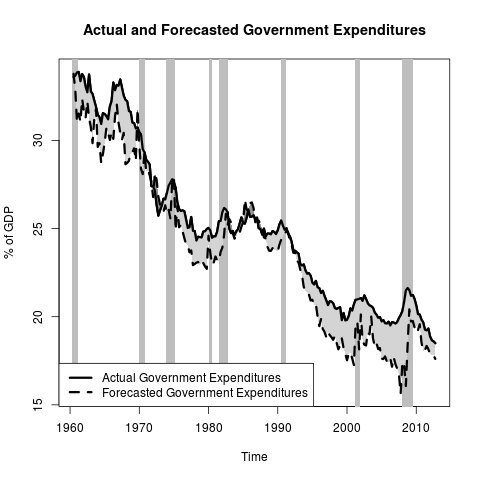
\includegraphics[width=0.45\textwidth, height=0.45\textheight]{pics/pred_gov.png} & 
    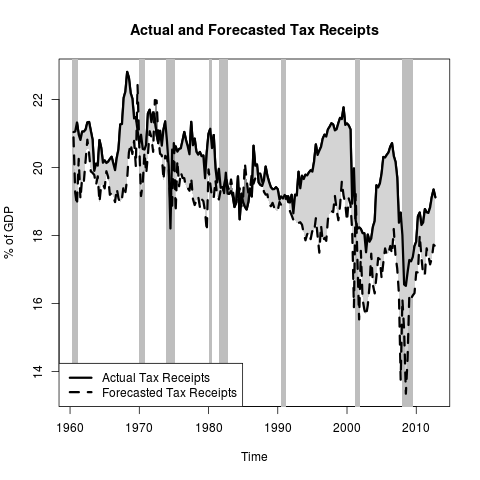
\includegraphics[width=0.45\textwidth, height=0.45\textheight]{pics/pred_tax.png} \\ 
    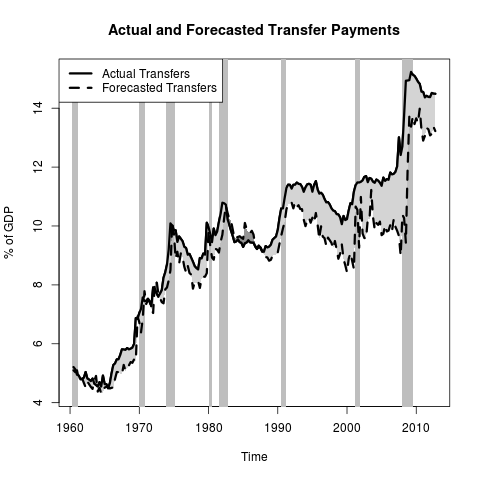
\includegraphics[width=0.45\textwidth, height=0.45\textheight]{pics/pred_transfers.png} & 
    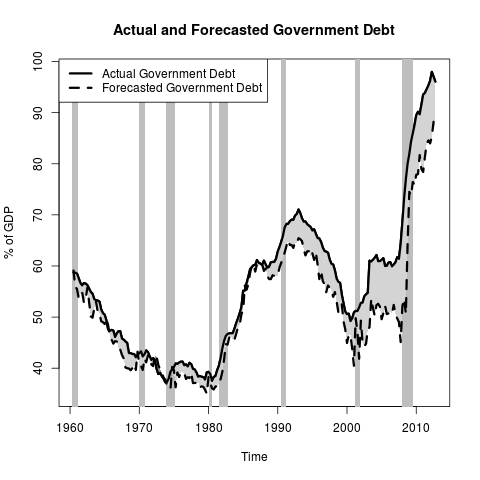
\includegraphics[width=0.45\textwidth, height=0.45\textheight]{pics/pred_debt.png} 
  \end{tabular}
}

\frame
{
  \ft{Fiscal Policy - Forecast Error}
  \begin{tabular}{cc}
    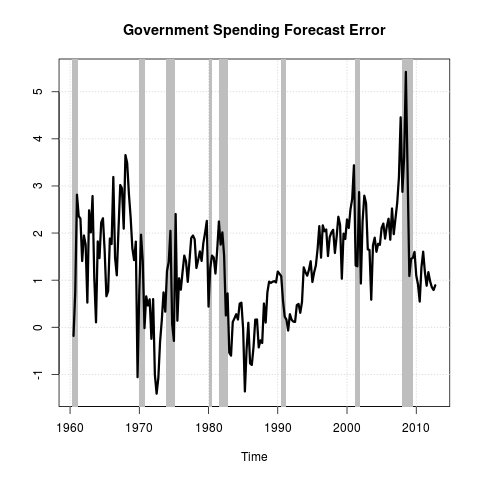
\includegraphics[width=0.45\textwidth, height=0.45\textheight]{pics/fe_gov.png} & 
    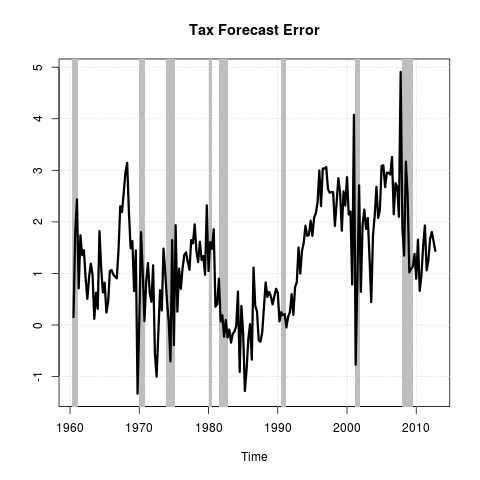
\includegraphics[width=0.45\textwidth, height=0.45\textheight]{pics/fe_tax.png} \\ 
    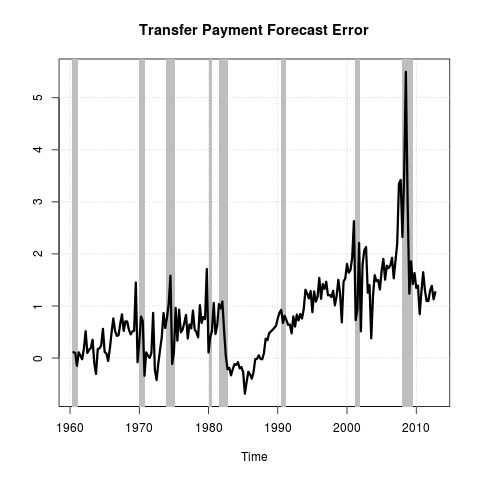
\includegraphics[width=0.45\textwidth, height=0.45\textheight]{pics/fe_transfers.png} & 
    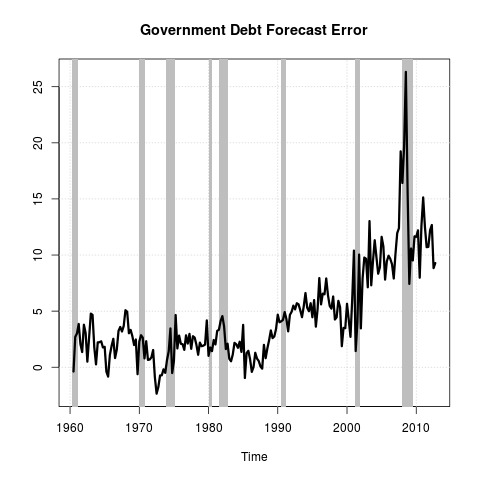
\includegraphics[width=0.45\textwidth, height=0.45\textheight]{pics/fe_debt.png} 
  \end{tabular}
}

\frame
{
  \ft{Fiscal Policy Uncertainty}
  \begin{tabular}{cc}
    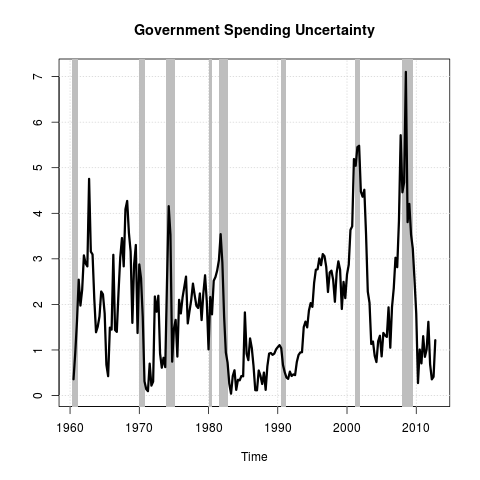
\includegraphics[width=0.45\textwidth, height=0.45\textheight]{pics/fpu_gov.png} & 
    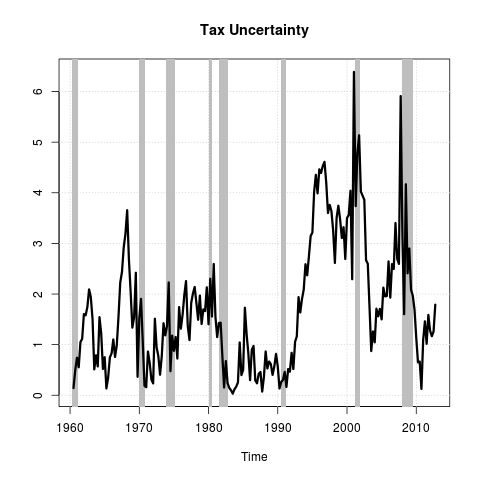
\includegraphics[width=0.45\textwidth, height=0.45\textheight]{pics/fpu_tax.png} \\ 
    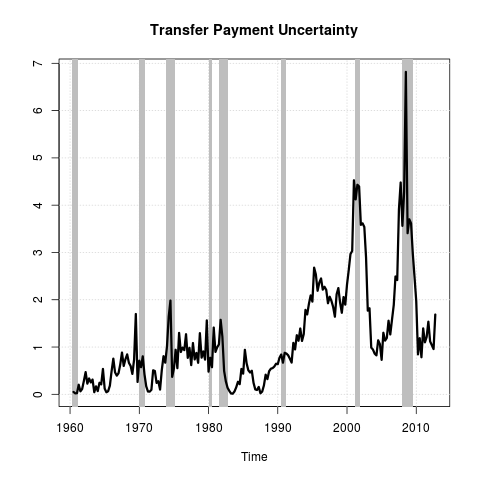
\includegraphics[width=0.45\textwidth, height=0.45\textheight]{pics/fpu_transfers.png} & 
    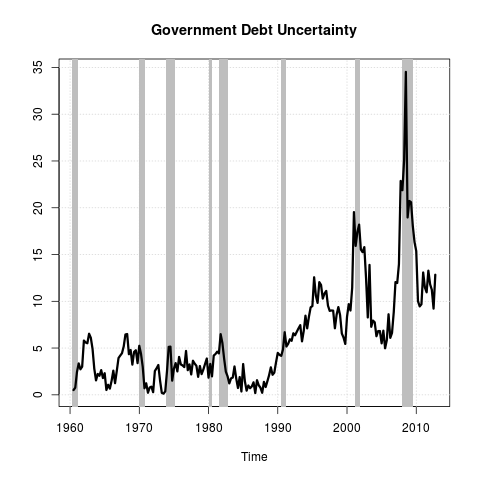
\includegraphics[width=0.45\textwidth, height=0.45\textheight]{pics/fpu_debt.png} 
  \end{tabular}
}

\frame
{
  \ft{Casual Observations}
  \bi
  \item Uncertainty concerning transfers and debt reached unprecedented levels during Great Recession.
    \bi
    \item Government expenditures uncertainty: Nearly 7\% of GDP
    \item Tax uncertainty: Nearly 6\% of GDP
    \item Transfers uncertainty: Nearly 7\% of GDP
    \item Government debt uncertainty: Nearly 35\% of GDP
    \ei
  \item Uncertainty seems to run up for several years preceding recessions:
    \bi
    \item Early 1980s, 2001, 2007.
    \item Not the rule though (eg: declines prior to 1970s, little volatility prior to 1991)
    \ei
  \item All are highly correlated with each other.
  \ei
}

\frame
{
  \ft{Fiscal Uncertainty Coincident Indicator}
  \bi
  \item Stock and Waston (1989) coincident indicator model
  \item Latent variable: General fiscal uncertainty
    \bdm \begin{array}{l} m_t = m_0 + A \lambda_t + e_t \\ [0.5pc]
\lambda_t = b_1 \lambda_{t-1} + b_2 \lambda_{t-2} + \upsilon_t\\ [0.5pc]
e_t = C e_{t-1} + \eta_t \end{array} \edm
   \item Notation:
     \bi
     \item $m_t$: 4x1 vector of fiscal uncertainty variables
     \item $\lambda_t$: general fiscal uncertainty
     \item $e_t$: ``unique'' component of fiscal uncertainty.
     \ei
   \ei
}

\frame
{
  \ft{Coincident Indicator: General Fiscal Uncertainty}
  \begin{center}
    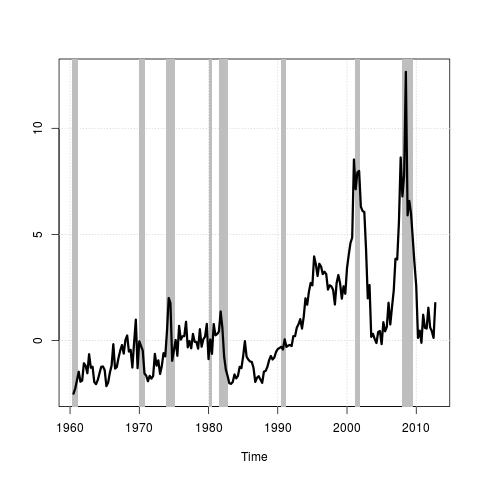
\includegraphics[width=0.8\textwidth]{pics/fpucoin.png}
  \end{center}
}

\frame
{
  \ft{Unique Fiscal Policy Uncertainty}
  \begin{tabular}{cc}
    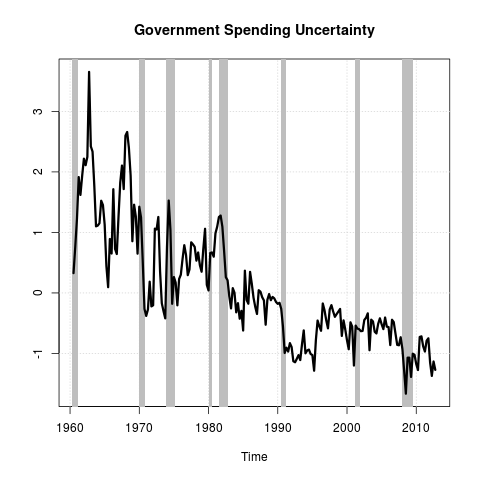
\includegraphics[width=0.45\textwidth, height=0.45\textheight]{pics/fpucoin_gov.png} & 
    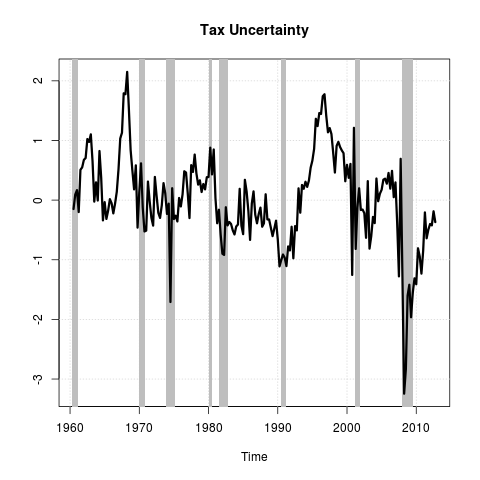
\includegraphics[width=0.45\textwidth, height=0.45\textheight]{pics/fpucoin_tax.png} \\ 
    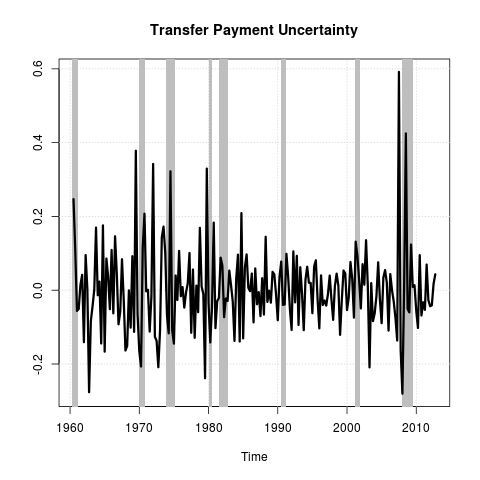
\includegraphics[width=0.45\textwidth, height=0.45\textheight]{pics/fpucoin_transfers.png} & 
    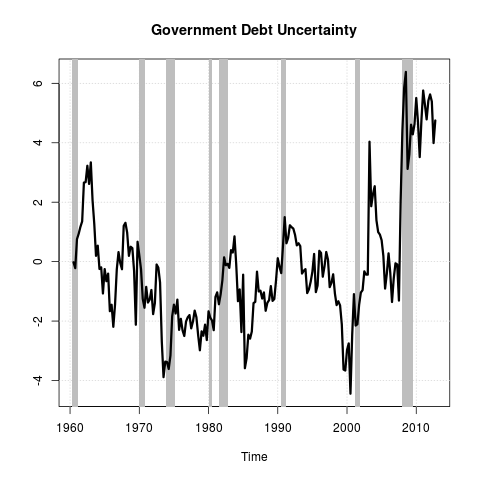
\includegraphics[width=0.45\textwidth, height=0.45\textheight]{pics/fpucoin_debt.png} 
  \end{tabular}
}



\frame
{
  \ft{Macroeconomic Consequences}
  \bi
  \item Answer this with a reduced form vector autoregression in:
    \be
    \item Real GDP
    \item Consumption
    \item Investment
    \item Unemployment
    \ee
  \item Augment explanatory variables with fiscal policy uncertainty variables (first lag)
  \item Consider VAR lag lengths: 1, 2, and 4.
  \item Consider learning gain parameters: $\gamma=0.01,~ 0.02,~0.03$.
  \ei
}

\frame[t]
{
  \ft{VAR Results: Real GDP}
\begin{scriptsize}
\begin{center}
\textbf{Dependent Variable: Real GDP}\\
\textbf{Learning Gain: $\gamma=0.02$}\\

\begin{tabular}{l|p{4pc}p{4pc}p{4pc}}\hline
 & \multicolumn{1}{c}{1 Lag} & \multicolumn{1}{c}{2 Lags} & \multicolumn{1}{c|}{4 Lags} \\ \hline 
\multirow{15}{*}{\begin{tabular}{l} Expenditure Uncertainty \\ (Standard Error)$^2$ \\ [0.2pc] Tax Uncertainty \\ (Standard Error) \\ [0.2pc] Transfers Uncertainty \\ (Standard Error) \\ [0.2pc] Debt Uncertainty \\ (Standard Error) \\ [0.2pc] Fiscal Uncertainty Index \hl{2} \\ (Standard Error) \hl{2} \\ [0.2pc] Joint F-test \hl{3} \\ [0.2pc] Adjusted R-square \\ AIC \\ BIC \end{tabular}}

& \multirow{15}{*}{\begin{tabular}{S[table-format=3.3]}
-0.093$^{}$ \\
(0.105) \\ [0.25pc]
0.886$^{}$ \\
(0.429) \\ [0.25pc]
0.404$^{}$ \\
(0.128) \\ [0.25pc]
0.014$^{}$ \\
(0.042) \\ [0.25pc]
-0.141$^{***}$ \hl{2} \\
(0.041) \hl{2} \\ [0.25pc]
\multicolumn{1}{S[table-format=3.1]}{4.0$^{***}$ \hl{3}} \\ [0.25pc]
\multicolumn{1}{S[table-format=1.3]}{0.250} \\ \multicolumn{1}{S[table-format=3.1]}{478.6} \\ \multicolumn{1}{S[table-format=3.1]}{535.4} \end{tabular}}

& \multirow{15}{*}{\begin{tabular}{S[table-format=3.3]}
-0.156$^{}$ \\
(0.127) \\ [0.25pc]
-0.680$^{}$ \\
(0.743) \\ [0.25pc]
0.475$^{}$ \\
(0.143) \\ [0.25pc]
0.006$^{}$ \\
(0.041) \\ [0.25pc]
-0.098$^{***}$ \hl{2} \\
(0.039) \hl{2} \\ [0.25pc]
\multicolumn{1}{S[table-format=3.1]}{2.1$^{*}$ \hl{3}} \\ [0.25pc]
\multicolumn{1}{S[table-format=1.3]}{0.343} \\ \multicolumn{1}{S[table-format=3.1]}{459.9} \\ \multicolumn{1}{S[table-format=3.1]}{550.1} \end{tabular}}

& \multirow{15}{*}{\begin{tabular}{S[table-format=3.3]}
-0.226$^{**}$ \\
(0.128) \\ [0.25pc]
-0.390$^{}$ \\
(0.704) \\ [0.25pc]
0.572$^{}$ \\
(0.123) \\ [0.25pc]
0.055$^{}$ \\
(0.047) \\ [0.25pc]
-0.117$^{***}$ \hl{2} \\
(0.039) \hl{2} \\ [0.25pc]
\multicolumn{1}{S[table-format=3.1]}{2.3$^{*}$ \hl{3}} \\ [0.25pc]
\multicolumn{1}{S[table-format=1.3]}{0.407} \\ \multicolumn{1}{S[table-format=3.1]}{454.0} \\ \multicolumn{1}{S[table-format=3.1]}{611.1} \end{tabular}}

\\  & & &   \\  & & & \\  & & & \\  & & &  \\  & & & \\  & & & \\ & & & \\ & & & \\ & & & \\  & & & \\  & & & \\  & & & \\  & & & \\ & & & \\  \hline 
\end{tabular}
\end{center}
\end{scriptsize}

\only<1>{\ \\}
\only<2>{\scriptsize{\textcolor{BrickRed}{\textbf{General fiscal uncertainty is followed by a decrease in real GDP}}}}
\only<3>{\scriptsize{\textcolor{BrickRed}{\textbf{At least one fiscal uncertainty variable influences real GDP}}}}
}

\frame
{
  \ft{Magnitude of the Impact}
  \bi
  \item Typical fluctuations in uncertainty over the sample period is not an important driver of business cycles.
     \bi
     \item Like Fern\'andez-Villiverde et. al. (2011a) and Born and Pfeifer (2011)
     \ei
  \item Buildup of fiscal uncertainty index from 2004 through 2007: Increase from 0.0 to 12.5.
  \item Coefficient on coincident index = -0.098.
  \item Impact on real GDP growth: 12.5 x (-0.098) = -1.2\%
  \ei
}

\frame[t]
{
  \ft{VAR Results: Consumption}
\begin{scriptsize}
\begin{center}
\textbf{Dependent Variable: Consumption}\\
\textbf{Learning Gain: $\gamma=0.02$}\\

\begin{tabular}{l|p{4pc}p{4pc}p{4pc}}\hline
 & \multicolumn{1}{c}{1 Lag} & \multicolumn{1}{c}{2 Lags} & \multicolumn{1}{c|}{4 Lags} \\ \hline 
\multirow{15}{*}{\begin{tabular}{l} Expenditure Uncertainty \\ (Standard Error)$^2$ \\ [0.2pc] Tax Uncertainty \\ (Standard Error) \\ [0.2pc] Transfers Uncertainty \\ (Standard Error) \\ [0.2pc] Debt Uncertainty \\ (Standard Error) \\ [0.2pc] Fiscal Uncertainty Index \hl{2} \\ (Standard Error) \hl{2} \\ [0.2pc] Joint F-test \hl{3} \\ [0.2pc] Adjusted R-square \\ AIC \\ BIC \end{tabular}}
& \multirow{15}{*}{\begin{tabular}{S[table-format=3.3]}
0.041$^{}$ \\
(0.067) \\ [0.25pc]
-0.051$^{}$ \\
(0.275) \\ [0.25pc]
0.028$^{}$ \\
(0.061) \\ [0.25pc]
-0.043$^{**}$ \\
(0.025) \\ [0.25pc]
-0.055$^{***}$ \hl{2} \\
(0.017) \hl{2} \\ [0.25pc]
\multicolumn{1}{S[table-format=3.1]}{2.7$^{**}$ \hl{3}} \\ [0.25pc]
\multicolumn{1}{S[table-format=1.3]}{0.980} \\ \multicolumn{1}{S[table-format=3.1]}{182.7} \\ \multicolumn{1}{S[table-format=3.1]}{239.6} \end{tabular}}
& \multirow{15}{*}{\begin{tabular}{S[table-format=3.3]}
-0.028$^{}$ \\
(0.071) \\ [0.25pc]
-0.588$^{*}$ \\
(0.413) \\ [0.25pc]
0.108$^{}$ \\
(0.071) \\ [0.25pc]
-0.032$^{}$ \\
(0.026) \\ [0.25pc]
-0.055$^{***}$ \hl{2} \\
(0.022) \hl{2} \\ [0.25pc]
\multicolumn{1}{S[table-format=3.1]}{2.1$^{*}$ \hl{3}} \\ [0.25pc]
\multicolumn{1}{S[table-format=1.3]}{0.980} \\ \multicolumn{1}{S[table-format=3.1]}{189.5} \\ \multicolumn{1}{S[table-format=3.1]}{279.7} \end{tabular}}
& \multirow{15}{*}{\begin{tabular}{S[table-format=3.3]}
-0.057$^{}$ \\
(0.059) \\ [0.25pc]
-0.653$^{*}$ \\
(0.401) \\ [0.25pc]
0.041$^{}$ \\
(0.071) \\ [0.25pc]
-0.024$^{}$ \\
(0.029) \\ [0.25pc]
-0.013$^{}$ \hl{2} \\
(0.026) \hl{2} \\ [0.25pc]
\multicolumn{1}{S[table-format=3.1]}{0.8$^{}$ \hl{3}} \\ [0.25pc]
\multicolumn{1}{S[table-format=1.3]}{0.981} \\ \multicolumn{1}{S[table-format=3.1]}{198.6} \\ \multicolumn{1}{S[table-format=3.1]}{355.7} \end{tabular}}
\\  & & &   \\  & & & \\  & & & \\  & & &  \\  & & & \\  & & & \\ & & & \\ & & & \\ & & & \\  & & & \\  & & & \\  & & & \\  & & & \\ & & & \\ & & & \\  \hline 
\end{tabular}
\end{center}
\end{scriptsize}

\only<1>{\ \\}
\only<2>{\scriptsize{\textcolor{BrickRed}{\textbf{General fiscal uncertainty is followed by a decrease in consumption}}}}
\only<3>{\scriptsize{\textcolor{BrickRed}{\textbf{At least one fiscal uncertainty variable influences consumption}}}}
}

\frame[t]
{
  \ft{VAR Results: Investment}
\begin{scriptsize}
\begin{center}
\textbf{Dependent Variable: Investment}\\
\textbf{Learning Gain: $\gamma=0.02$}\\

\begin{tabular}{l|p{4pc}p{4pc}p{4pc}}\hline
 & \multicolumn{1}{c}{1 Lag} & \multicolumn{1}{c}{2 Lags} & \multicolumn{1}{c|}{4 Lags} \\ \hline 
\multirow{15}{*}{\begin{tabular}{l} Expenditure Uncertainty \\ (Standard Error)$^2$ \\ [0.2pc] Tax Uncertainty \\ (Standard Error) \\ [0.2pc] Transfers Uncertainty \\ (Standard Error) \\ [0.2pc] Debt Uncertainty \\ (Standard Error) \\ [0.2pc] Fiscal Uncertainty Index \hl{2} \\ (Standard Error) \hl{2} \\ [0.2pc] Joint F-test \hl{3} \\ [0.2pc] Adjusted R-square \\ AIC \\ BIC \end{tabular}}

& \multirow{15}{*}{\begin{tabular}{S[table-format=3.3]}
-0.096$^{*}$ \\
(0.062) \\ [0.25pc]
0.702$^{}$ \\
(0.329) \\ [0.25pc]
0.416$^{}$ \\
(0.084) \\ [0.25pc]
0.064$^{}$ \\
(0.034) \\ [0.25pc]
-0.104$^{***}$ \hl{2} \\
(0.033) \hl{2} \\ [0.25pc]
\multicolumn{1}{S[table-format=3.1]}{6.4$^{***}$ \hl{3}} \\ [0.25pc]
\multicolumn{1}{S[table-format=1.3]}{0.945} \\ \multicolumn{1}{S[table-format=3.1]}{296.6} \\ \multicolumn{1}{S[table-format=3.1]}{353.4} \end{tabular}}
& \multirow{15}{*}{\begin{tabular}{S[table-format=3.3]}
-0.061$^{}$ \\
(0.078) \\ [0.25pc]
-0.096$^{}$ \\
(0.371) \\ [0.25pc]
0.326$^{}$ \\
(0.112) \\ [0.25pc]
0.044$^{}$ \\
(0.027) \\ [0.25pc]
-0.048$^{**}$ \hl{2} \\
(0.029) \hl{2} \\ [0.25pc]
\multicolumn{1}{S[table-format=3.1]}{2.5$^{**}$ \hl{3}} \\ [0.25pc]
\multicolumn{1}{S[table-format=1.3]}{0.958} \\ \multicolumn{1}{S[table-format=3.1]}{251.9} \\ \multicolumn{1}{S[table-format=3.1]}{342.1} \end{tabular}}
& \multirow{15}{*}{\begin{tabular}{S[table-format=3.3]}
-0.085$^{}$ \\
(0.088) \\ [0.25pc]
0.247$^{}$ \\
(0.368) \\ [0.25pc]
0.401$^{}$ \\
(0.090) \\ [0.25pc]
0.075$^{}$ \\
(0.025) \\ [0.25pc]
-0.077$^{***}$ \hl{2} \\
(0.024) \hl{2} \\ [0.25pc]
\multicolumn{1}{S[table-format=3.1]}{3.5$^{***}$ \hl{3}} \\ [0.25pc]
\multicolumn{1}{S[table-format=1.3]}{0.962} \\ \multicolumn{1}{S[table-format=3.1]}{245.7} \\ \multicolumn{1}{S[table-format=3.1]}{402.8} \end{tabular}}

\\  & & &   \\  & & & \\  & & & \\  & & &  \\  & & & \\  & & & \\ & & & \\ & & & \\ & & & \\  & & & \\  & & & \\  & & & \\  & & & \\ & & & \\ & & & \\  \hline 
\end{tabular}
\end{center}
\end{scriptsize}

\only<1>{\ \\}
\only<2>{\scriptsize{\textcolor{BrickRed}{\textbf{General fiscal uncertainty is followed by a decrease in investment}}}}
\only<3>{\scriptsize{\textcolor{BrickRed}{\textbf{At least one fiscal uncertainty variable influences investment}}}}
}


\frame[t]
{
  \ft{VAR Results: Investment}
\begin{scriptsize}
\begin{center}
\textbf{Dependent Variable: Unemployment}\\
\textbf{Learning Gain: $\gamma=0.02$}\\

\begin{tabular}{l|p{4pc}p{4pc}p{4pc}}\hline
 & \multicolumn{1}{c}{1 Lag} & \multicolumn{1}{c}{2 Lags} & \multicolumn{1}{c|}{4 Lags} \\ \hline 
\multirow{15}{*}{\begin{tabular}{l} Expenditure Uncertainty \\ (Standard Error)$^2$ \\ [0.2pc] Tax Uncertainty \\ (Standard Error) \\ [0.2pc] Transfers Uncertainty \hl{2} \\ (Standard Error) \hl{2} \\ [0.2pc] Debt Uncertainty \\ (Standard Error) \\ [0.2pc] Fiscal Uncertainty Index \\ (Standard Error) \\ [0.2pc] Joint F-test \hl{3} \\ [0.2pc] Adjusted R-square \\ AIC \\ BIC \end{tabular}}
& \multirow{15}{*}{\begin{tabular}{S[table-format=3.3]}
0.031$^{}$ \\
(0.035) \\ [0.25pc]
-0.260$^{*}$ \\
(0.194) \\ [0.25pc]
-0.178$^{***}$ \hl{2} \\
(0.048) \hl{2} \\ [0.25pc]
-0.006$^{}$ \\
(0.024) \\ [0.25pc]
0.077$^{}$ \\
(0.020) \\ [0.25pc]
\multicolumn{1}{S[table-format=3.1]}{9.0$^{***}$ \hl{3}} \\ [0.25pc]
\multicolumn{1}{S[table-format=1.3]}{0.979} \\ \multicolumn{1}{S[table-format=3.1]}{11.1} \\ \multicolumn{1}{S[table-format=3.1]}{67.9} \end{tabular}}
& \multirow{15}{*}{\begin{tabular}{S[table-format=3.3]}
0.004$^{}$ \\
(0.046) \\ [0.25pc]
-0.026$^{}$ \\
(0.193) \\ [0.25pc]
-0.127$^{***}$ \hl{2} \\
(0.043) \hl{2} \\ [0.25pc]
0.013$^{}$ \\
(0.017) \\ [0.25pc]
0.040$^{}$ \\
(0.018) \\ [0.25pc]
\multicolumn{1}{S[table-format=3.1]}{2.3$^{**}$ \hl{3}} \\ [0.25pc]
\multicolumn{1}{S[table-format=1.3]}{0.983} \\ \multicolumn{1}{S[table-format=3.1]}{-22.5} \\ \multicolumn{1}{S[table-format=3.1]}{67.7} \end{tabular}}
& \multirow{15}{*}{\begin{tabular}{S[table-format=3.3]}
0.016$^{}$ \\
(0.042) \\ [0.25pc]
-0.128$^{}$ \\
(0.215) \\ [0.25pc]
-0.147$^{***}$ \hl{2} \\
(0.045) \hl{2} \\ [0.25pc]
0.010$^{}$ \\
(0.017) \\ [0.25pc]
0.056$^{}$ \\
(0.019) \\ [0.25pc]
\multicolumn{1}{S[table-format=3.1]}{2.2$^{*}$ \hl{3}} \\ [0.25pc]
\multicolumn{1}{S[table-format=1.3]}{0.982} \\ \multicolumn{1}{S[table-format=3.1]}{-0.9} \\ \multicolumn{1}{S[table-format=3.1]}{156.2} \end{tabular}}



\\  & & &   \\  & & & \\  & & & \\  & & &  \\  & & & \\  & & & \\ & & & \\ & & & \\ & & & \\  & & & \\  & & & \\  & & & \\  & & & \\ & & & \\ & & & \\  \hline 
\end{tabular}
\end{center}
\end{scriptsize}

\only<1>{\ \\}
\only<2>{\scriptsize{\textcolor{BrickRed}{\textbf{Transfers uncertainty is followed by a \textit{decrease in unemployment}}}}}
\only<3>{\scriptsize{\textcolor{BrickRed}{\textbf{At least one fiscal uncertainty variable influences unemployment}}}}
}



\frame
{
  \ft{Impact on Unemployment}
  \bi
  \item Labor supply story?  Uncertainty on transfers increases job search effort?
    \bi
    \item Farber and Velletta (2013): Extension on unemployment benefits leads to (small) increases in unemployment / duration.
    \ei

  \item Magnitude
    \bi
    \item Buildup of fiscal uncertainty index from 2004 through 2007: Increase from -0.01 to 0.06.
    \item Coefficient on coincident index = -0.127.
    \item Impact on unemployment rate: 0.07 x (-0.127) = -0.089\%
    \ei
  \ei
}


\frame
{
  \ft{Conclusions}
  Fiscal Uncertainty Reduces Economic Activity

  \bi
  \item General measure for fiscal uncertainty associated with:
    \bi
    \item lower real GDP,
    \item lower consumption,
    \item lower investment.
    \ei
 
  \item Less robust to specification (not shown):
    \bi
    \item Expenditures uncertainty $\rightarrow$ lower investment and real GDP.
    \item Tax uncertainty $\rightarrow$ lower consumption and real GDP.
    \ei

 \item Transfers uncertainty associated with \textit{lower unemployment}.
    \bi
    \item Statistically significant
    \item Quantitatively tiny.
    \ei
  \ei

}








\end{document}

